\documentclass[10pt]{article}
\usepackage[T1,T2A]{fontenc}
\usepackage[english, russian]{babel}
\usepackage[left=1cm, right=1cm, top=1cm]{geometry}
\usepackage{amsmath}
\usepackage{graphicx}
\usepackage{titling}
\usepackage{graphicx}

\setlength{\droptitle}{-2cm}
 
\title{ИДЗ 19.1 ВАРИАНТ 3}
\author{Гаврилин Олег}

\begin{document}
\maketitle

а-б)
\begin{center}
\begin{tabular}{ |c|c|c|c|c|c|c| }
\hline
Интервал & Середина интервала $x_i$ & Частота $f_i$ & $w_i=\frac{f_i}{n}$ & $w_i^{HAK}$ & $x_if_i$ & $x_i^2f_i$ \\
182.0 - 188.0 & 185.0 & 8 & 0.08 & 0.08 & 1480.0 & 273800.0 \\
188.0 - 194.0 & 191.0 & 10 & 0.1 & 0.18 & 1910.0 & 364810.0 \\
194.0 - 200.0 & 197.0 & 9 & 0.09 & 0.27 & 1773.0 & 349281.0 \\
200.0 - 206.0 & 203.0 & 15 & 0.15 & 0.42 & 3045.0 & 618135.0 \\
206.0 - 212.0 & 209.0 & 16 & 0.16 & 0.58 & 3344.0 & 698896.0 \\
212.0 - 218.0 & 215.0 & 14 & 0.14 & 0.72 & 3010.0 & 647150.0 \\
218.0 - 224.0 & 221.0 & 9 & 0.09 & 0.81 & 1989.0 & 439569.0 \\
224.0 - 230.0 & 227.0 & 10 & 0.1 & 0.91 & 2270.0 & 515290.0 \\
230.0 - 236.0 & 233.0 & 9 & 0.09 & 1.0 & 2097.0 & 488601.0 \\
\quad & $\sum$ & $n=100$ & 1 & \quad & 20918.0 & 4395532.0 \\
\hline
\end{tabular}
\end{center}

в)

\centerline{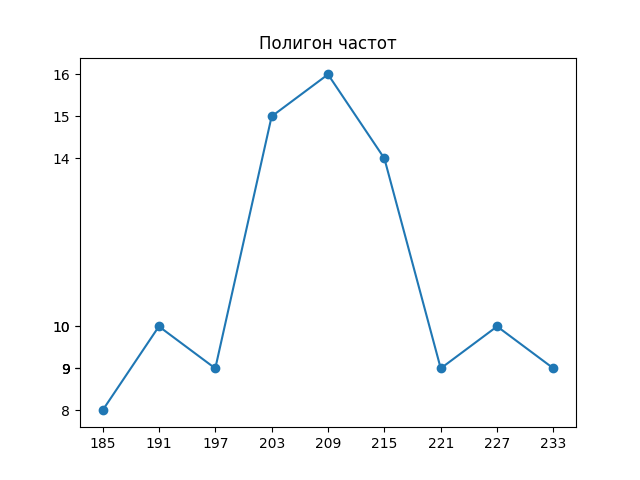
\includegraphics[scale=0.7]{1.png}}

\centerline{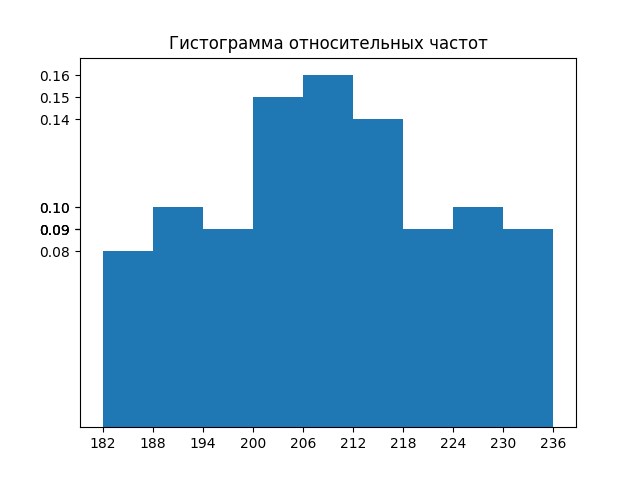
\includegraphics[scale=0.7]{2.png}}

\centerline{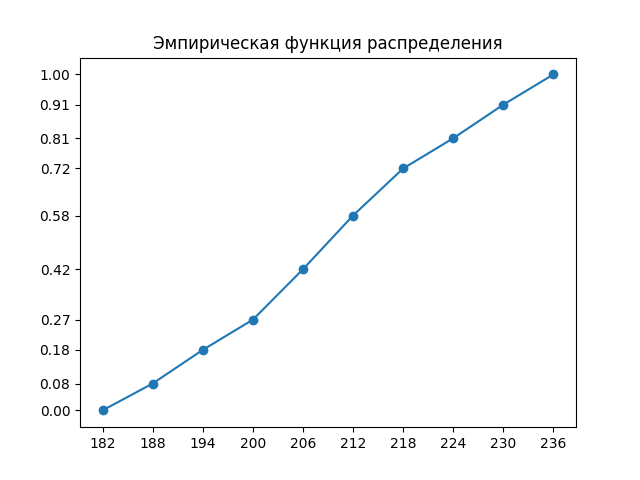
\includegraphics[scale=0.7]{3.png}}

г)

Вычислим среднюю арифметическую:
\[\overline{x}=\frac{\sum x_i f_i}{n}=209.18\]
\[D=\frac{\sum x_i^2 f_i}{n} - \overline{x}=199.05\]

д)

Найдем значение теоретических частот $f_i^T$ используя формулу:
$f_i^T=\frac{hn}{\sigma}f(t)$

где $f(t)=\frac{1}{\sqrt{2\pi}}e^{-\frac{t^2}{2}}, t=\frac{x_i-\overline{x}}{\sigma}$
$\sigma=\sqrt{D}=14.11$

Расчетная таблица
\begin{center}
\begin{tabular}{ |c|c|c|c| }
\hline
$x_i$ & $t_i$ & $f(t_i)$ & $f_i^T$ \\
185.0 & -1.71 & 0.09 & 4 \\
191.0 & -1.29 & 0.17 & 7 \\
197.0 & -0.86 & 0.27 & 12 \\
203.0 & -0.44 & 0.36 & 15 \\
209.0 & -0.01 & 0.4 & 17 \\
215.0 & 0.41 & 0.37 & 16 \\
221.0 & 0.84 & 0.28 & 12 \\
227.0 & 1.26 & 0.18 & 8 \\
233.0 & 1.69 & 0.1 & 4 \\
\hline
\end{tabular}
\end{center}

Расчетное значение критерия вычислим по формуле:
$\chi^2=\sum_{i=1}^l\frac{(f_i-f^T_i)^2}{f_i^T}$.

где $l$ - количество интервалов\\

Расчетная таблица
\begin{center}
\begin{tabular}{ |c|c|c| }
\hline
$f_i$ & $f_i^T$ & $\chi^2$ \\
0.09 & 4 & 4.0 \\
0.17 & 7 & 1.29 \\
0.27 & 12 & 0.75 \\
0.36 & 15 & 0.0 \\
0.4 & 17 & 0.06 \\
0.37 & 16 & 0.25 \\
0.28 & 12 & 0.75 \\
0.18 & 8 & 0.5 \\
0.1 & 4 & 6.25 \\
\hline
\end{tabular}
\end{center}

Таким образом $\chi^2 = 13.84$.

Теоретическое значение критерия возьмем из таблицы. Оно равно $14.4$.
Таким образом $\chi ^ 2 = 13.84 < 14.4$, то есть на уровне значимости
$\alpha=0.025$ принимаем нулевую гипотезу о том, что генеральная совокупность,
из которой извлечена выборка, имеет нормальное распределение.

е)

Доверительный интервал истинного значения генеральной средней вычислим по формуле
\[\overline{x}-\frac{t_{\gamma}\sigma}{\sqrt{n}} < \tilde{x} <
\overline{x} + \frac{t_{\gamma}\sigma}{\sqrt{n}}\]
Выберем уровень доверительной вероятности $\gamma = 0.05$.
По таблице распределения Стъюдента находим $t_{\gamma}=2.31$.\\

Вычислим точность оценки:
\[\frac{t_{\gamma}\sigma}{\sqrt{n}} \approx 3.26\]

Таким образом
\[205.92 < \tilde{x} < 212.44\]

с вероятностью $95\%$ данный интервал накроет истинное значение $\tilde{x}$
генеральной средней.\\

Доверительный интервал для генерального среднего квадратического отклонения
определяется по формуле
\[\frac{\sqrt{2n}}{\sqrt{2n}-3+t_{\gamma}}\sigma<\tilde{\sigma}<
\frac{\sqrt{2n}}{\sqrt{2n}-3-t_{\gamma}}\sigma\]

Таким образом
\[12.21 < \tilde{\sigma} < 17.02\]

с вероятностью $95\%$ данный интервал накроет истинное значение $\tilde{\sigma}$
генерального среднего квадратического отклонения.


\end{document}